
\chapter{Montaje del Hardware y el Servicio Web}

\setlength{\parindent}{5ex}En este capitulo se va a explicar como se ha montado todo este sistema, así como una explicación de sus diferentes piezas y la función que realiza cada una de ellas tanto en la parte hardware como en la parte software.
También se realizara un estudio del coste de todos los materiales, así como el mantenimiento y consumo de estos.

\setlength{\parindent}{0ex}Esta es la estructura que se seguiremos para el montaje de la aplicación:

\begin{figure}[!h]
	\centering
	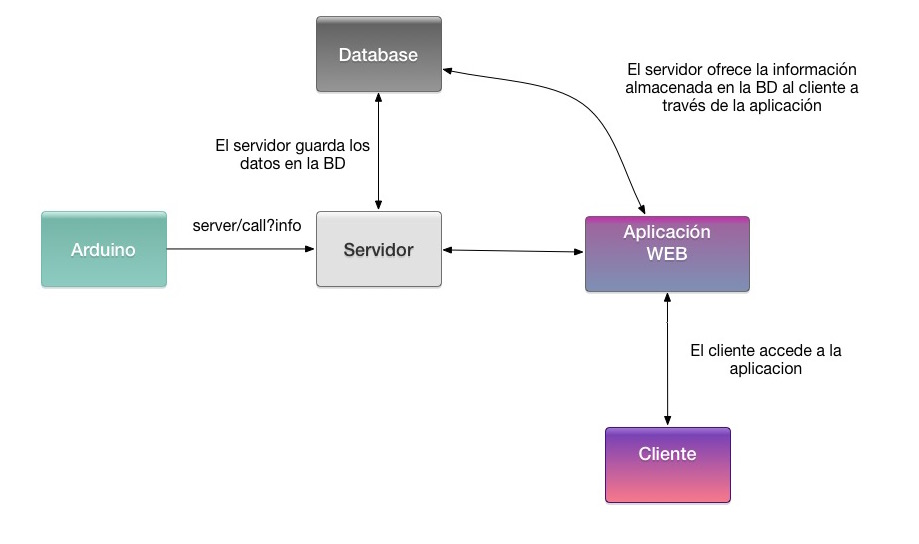
\includegraphics[width=0.9\linewidth]{figuras/montage1}
	\caption{Diagrama de montaje del proyecto}
	\label{fig:imgmontage1}
\end{figure}

En la \textbf{Figura \ref{fig:imgmontage1}} se puede observar el diagrama de montaje del proyecto en que función realizan las diferentes partes, desde el modulo hasta la información que podrá visualizar el cliente.

\section{Material}

\setlength{\parindent}{0ex}Para este proyecto se ha utilizado el siguiente material:\\

\textbf{Arduino Due:} Es la Controladora que se encarga de recibir la información y procesarla para enviarla al servidor.

\begin{figure}[!h]
	\centering
	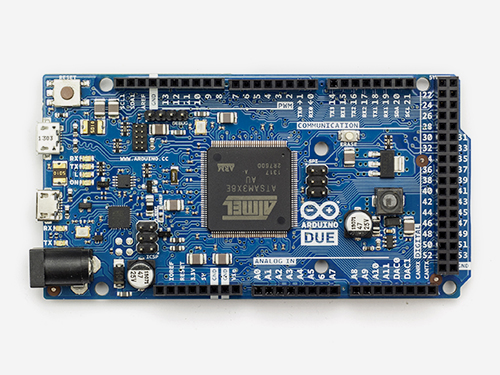
\includegraphics[width=0.4\linewidth]{figuras/arddue}
	\caption{Microcontroladora Arduino DUE}
	\label{fig:imgdue}
\end{figure}

\setlength{\parindent}{0ex}\textbf{Ethernet shield:} Es una Shield que permite a la micro controladora conectarse a la red.

\begin{figure}[!h]
	\centering
	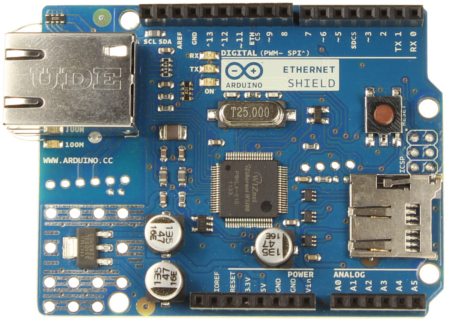
\includegraphics[width=0.3\linewidth]{figuras/ethshi}
	\caption{Ethernet shield}
	\label{fig:imgethshi}
\end{figure}

\setlength{\parindent}{0ex}\textbf{Modulo GPS NEO6mv2: }Es un módulo el cual contiene un GPS que una vez este conectado al satélite enviara información de la geolocalización.

	\begin{figure}[!h]
		\centering
		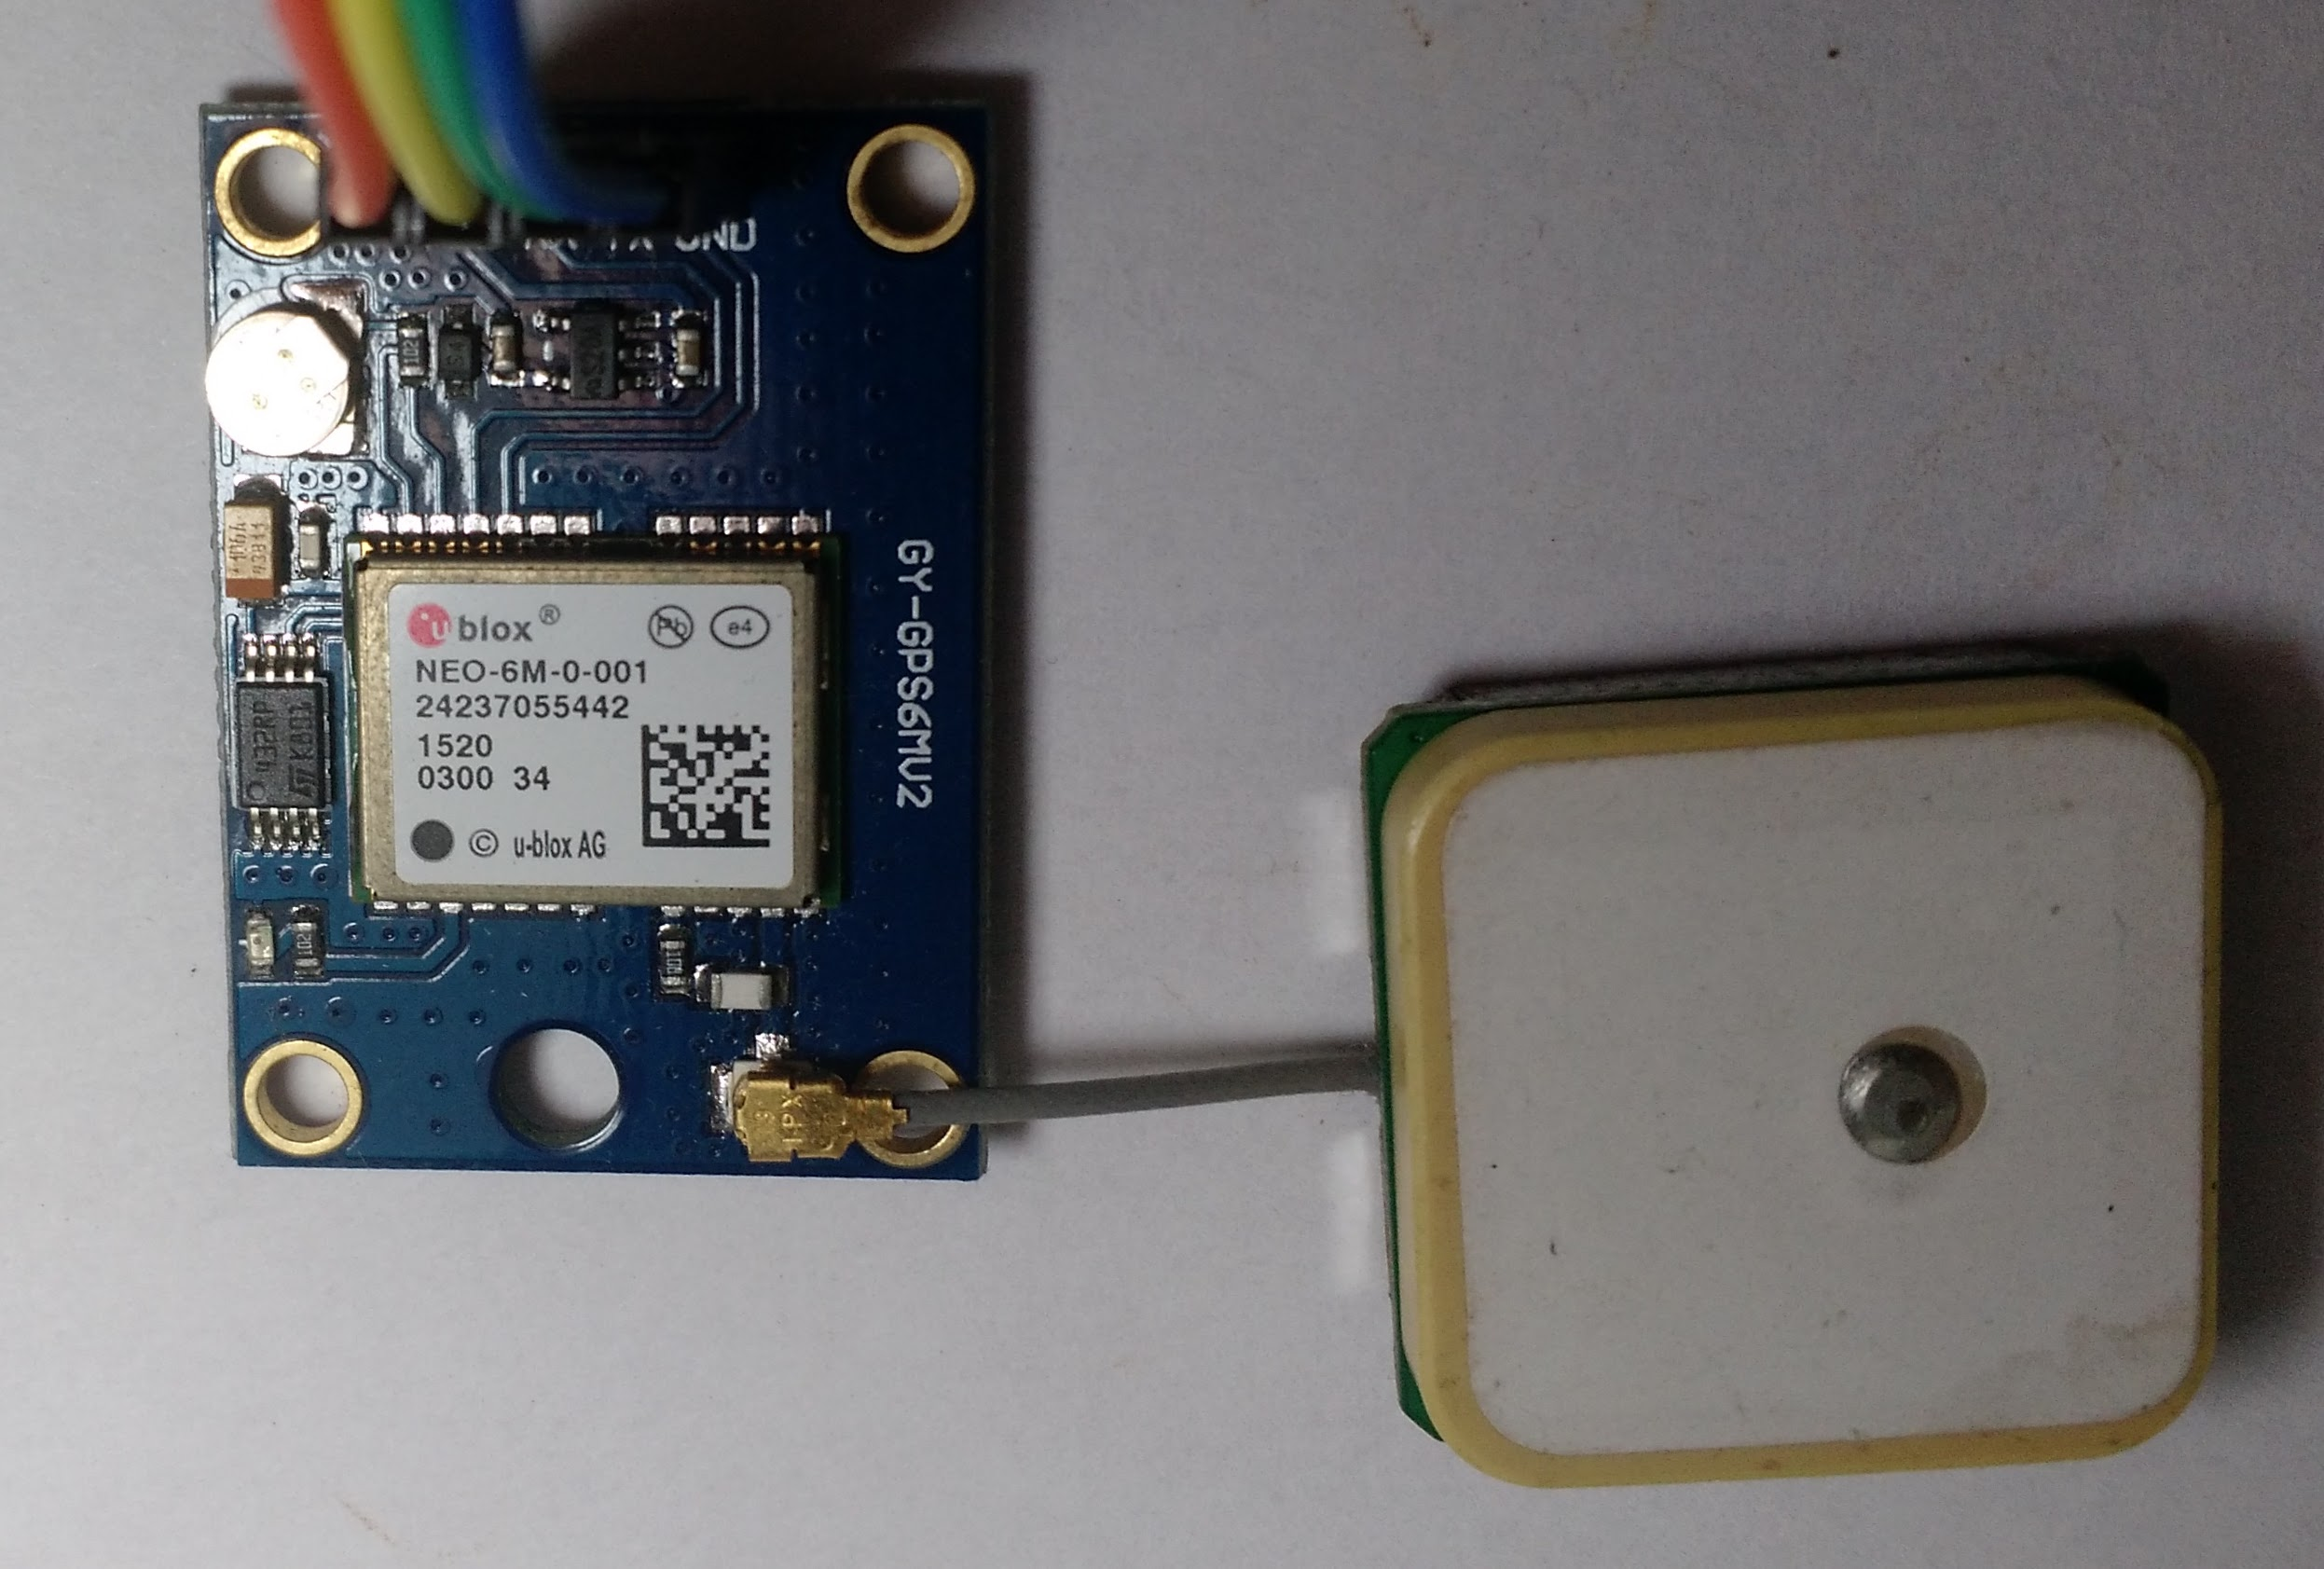
\includegraphics[width=0.6\linewidth]{figuras/neo6mv2}
		\caption{Sensor de Temperatura y Humedad DHT11}
		\label{fig:dht11}
	\end{figure}


\setlength{\parindent}{0ex}\textbf{Sensores:} Un conjunto de sensores que permitirá la obtención de los valores ambientales del entrono donde este instalado el nodo.

Estos sensores son:
	\clearpage
\begin{itemize}
	\item \textbf{DHT11} Es el sensor de Humedad y temperatura de Adafruit recogerá estos datos climáticos del ambiente.
	
	\begin{figure}[!h]
		\centering
		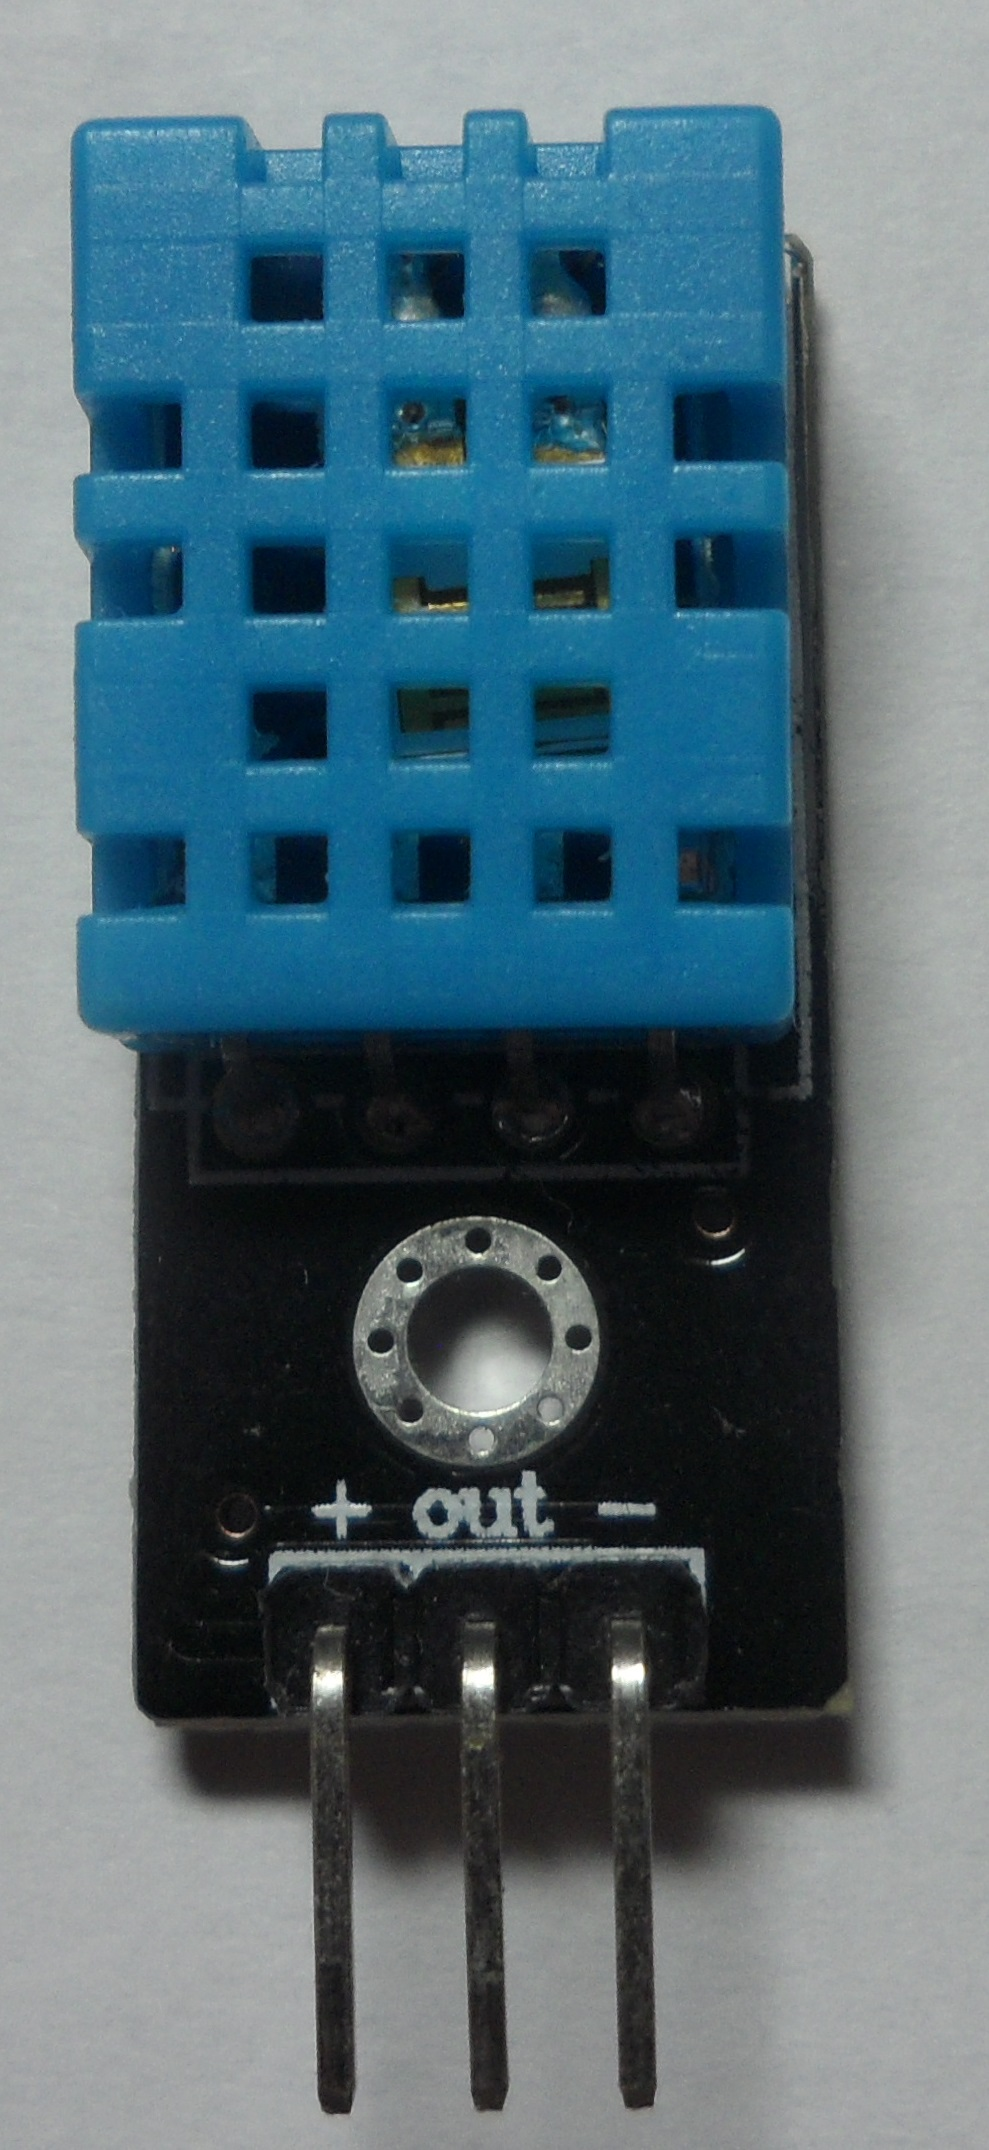
\includegraphics[width=0.2\linewidth]{figuras/dht11}
		\caption{Sensor de Temperatura y Humedad DHT11}
		\label{fig:dht11}
	\end{figure}

	
	\item \textbf{Sensor de gas CO MQ-7 y el chipset LM393} el que se utilizara para la medición de gases en el ambiente.
		\begin{figure}[!h]
			\centering
			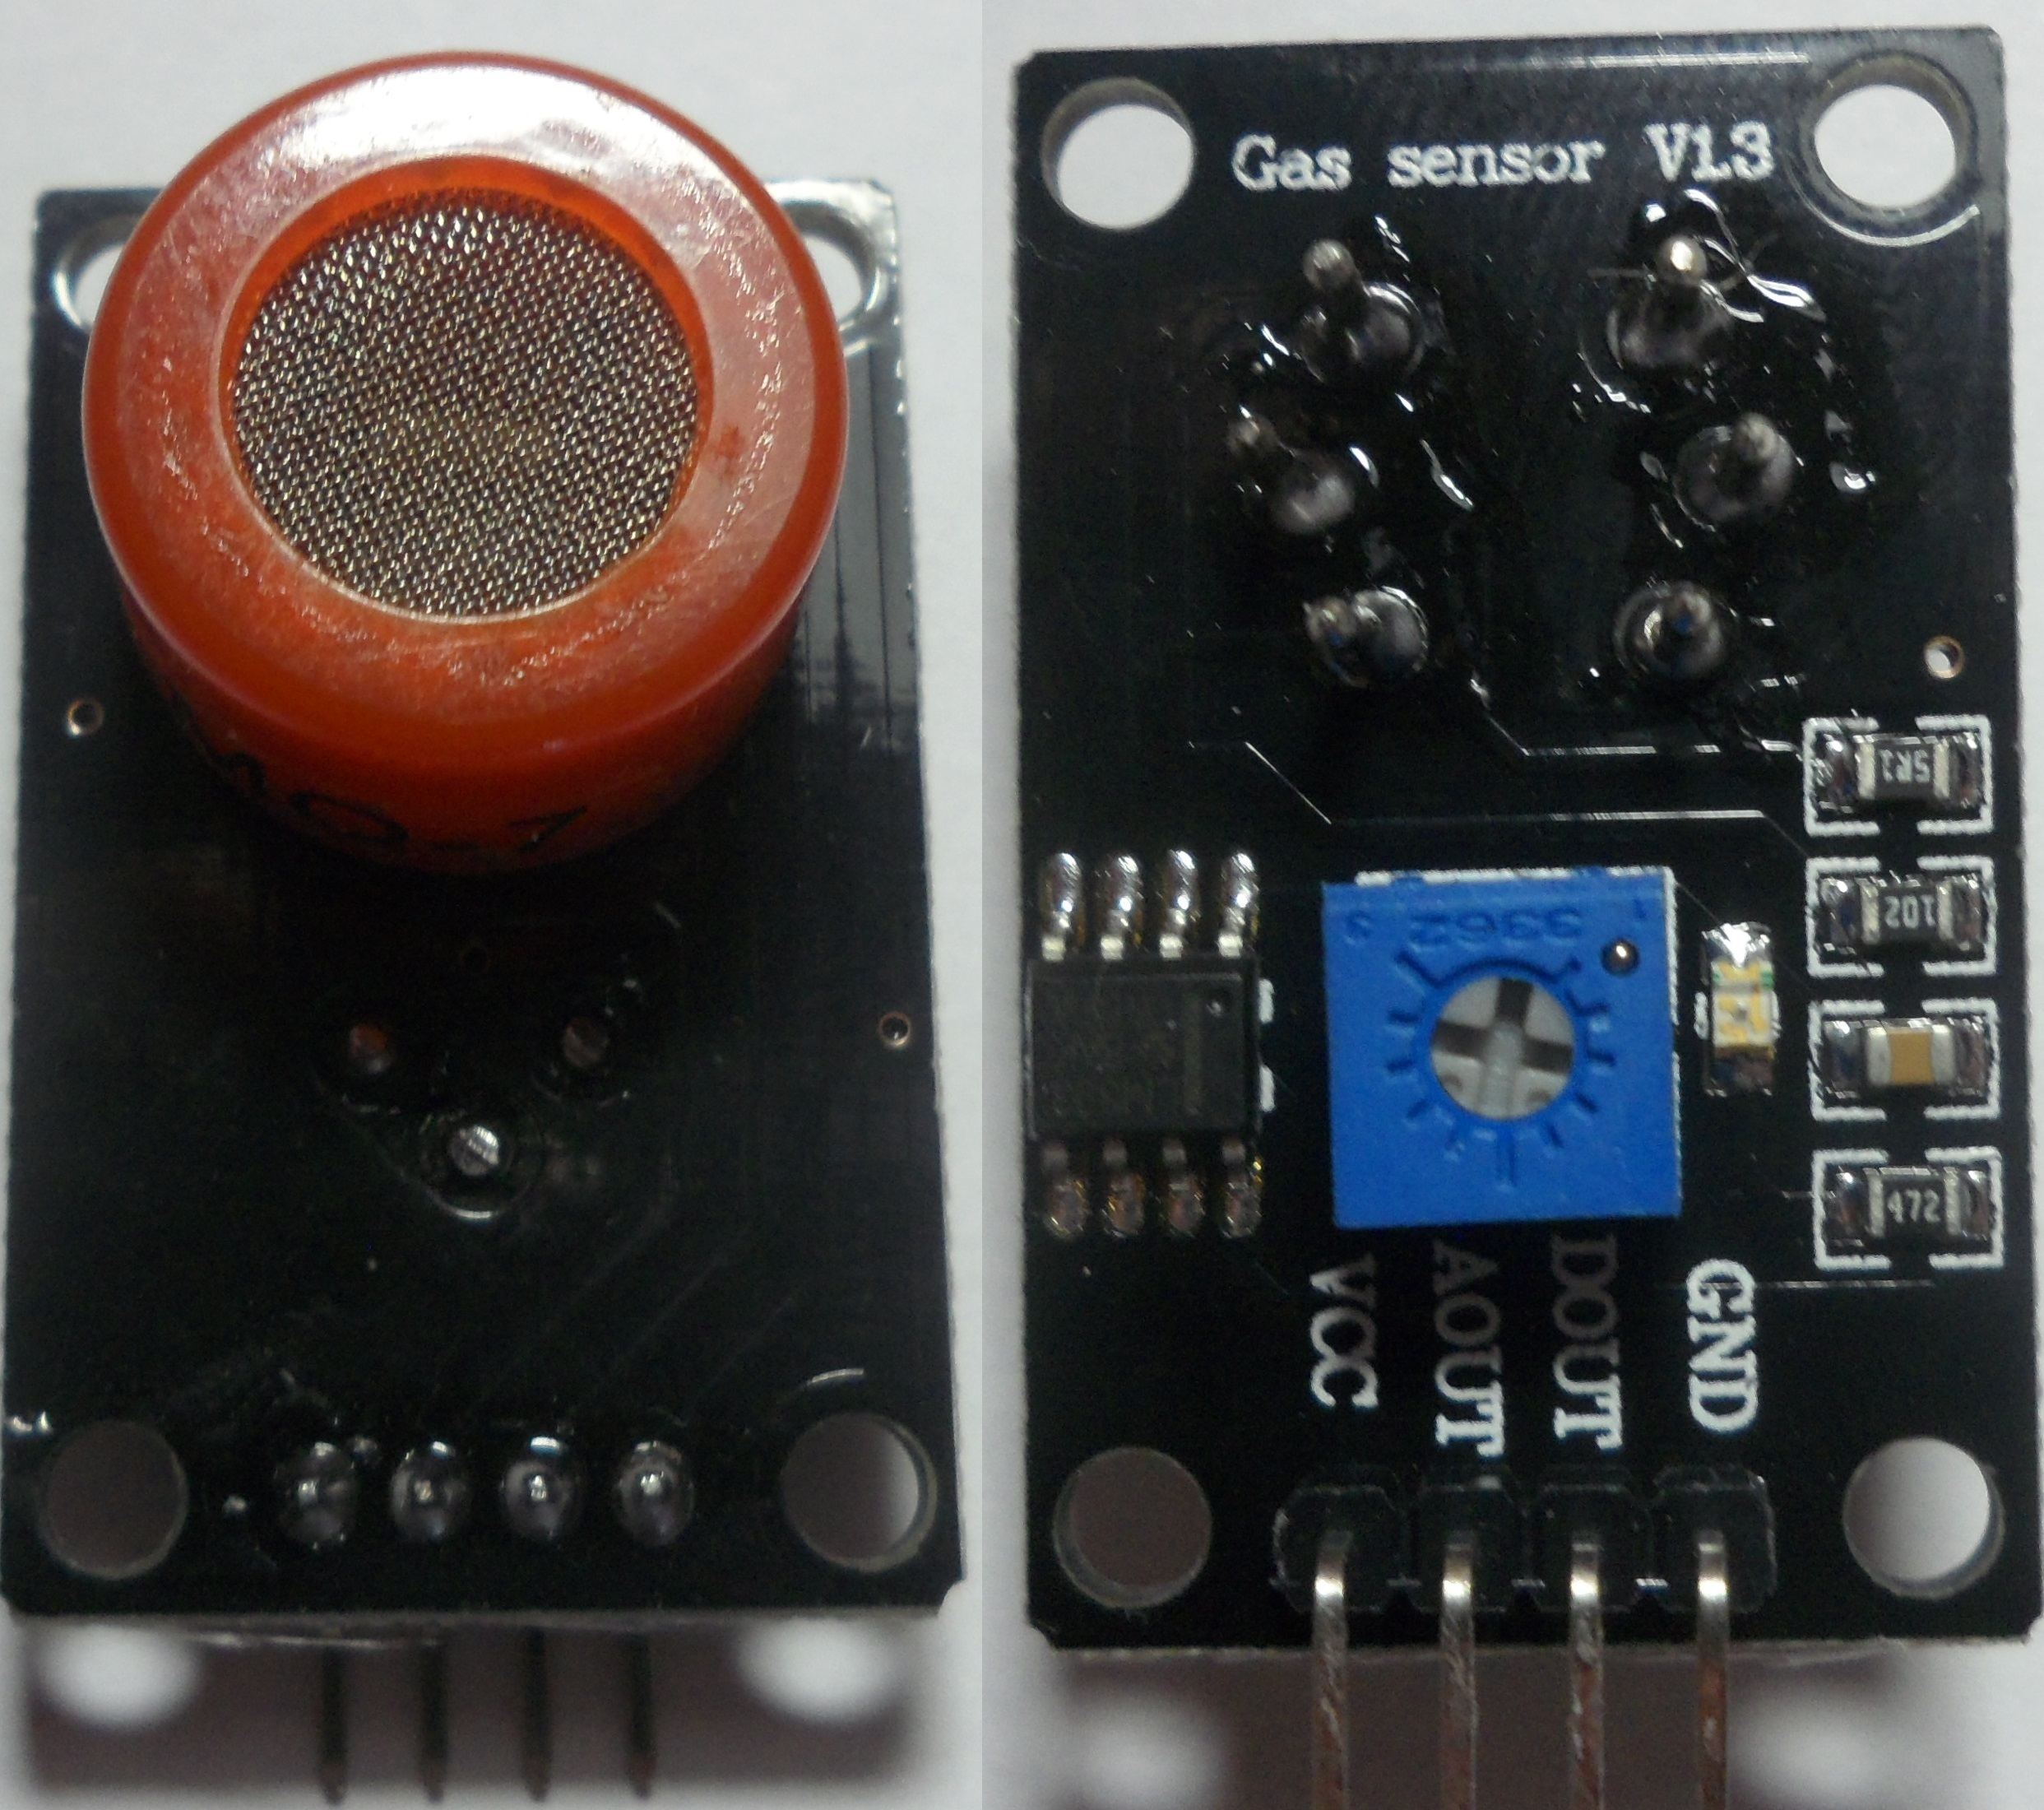
\includegraphics[width=0.4\linewidth]{figuras/gasen}
			\caption{Sensor de Mesura de Gas CO MQ-7}
			\label{fig:dht11}
		\end{figure}
	
	\item \textbf{Sensor luz y sonido} el cual también utiliza el chipset LM393 medirá la contaminación lumínica y acústica.
	

	\begin{figure}[!h]
		\centering
		\subfloat[Sensor de Luminosidad]{
			\label{f:luz}
			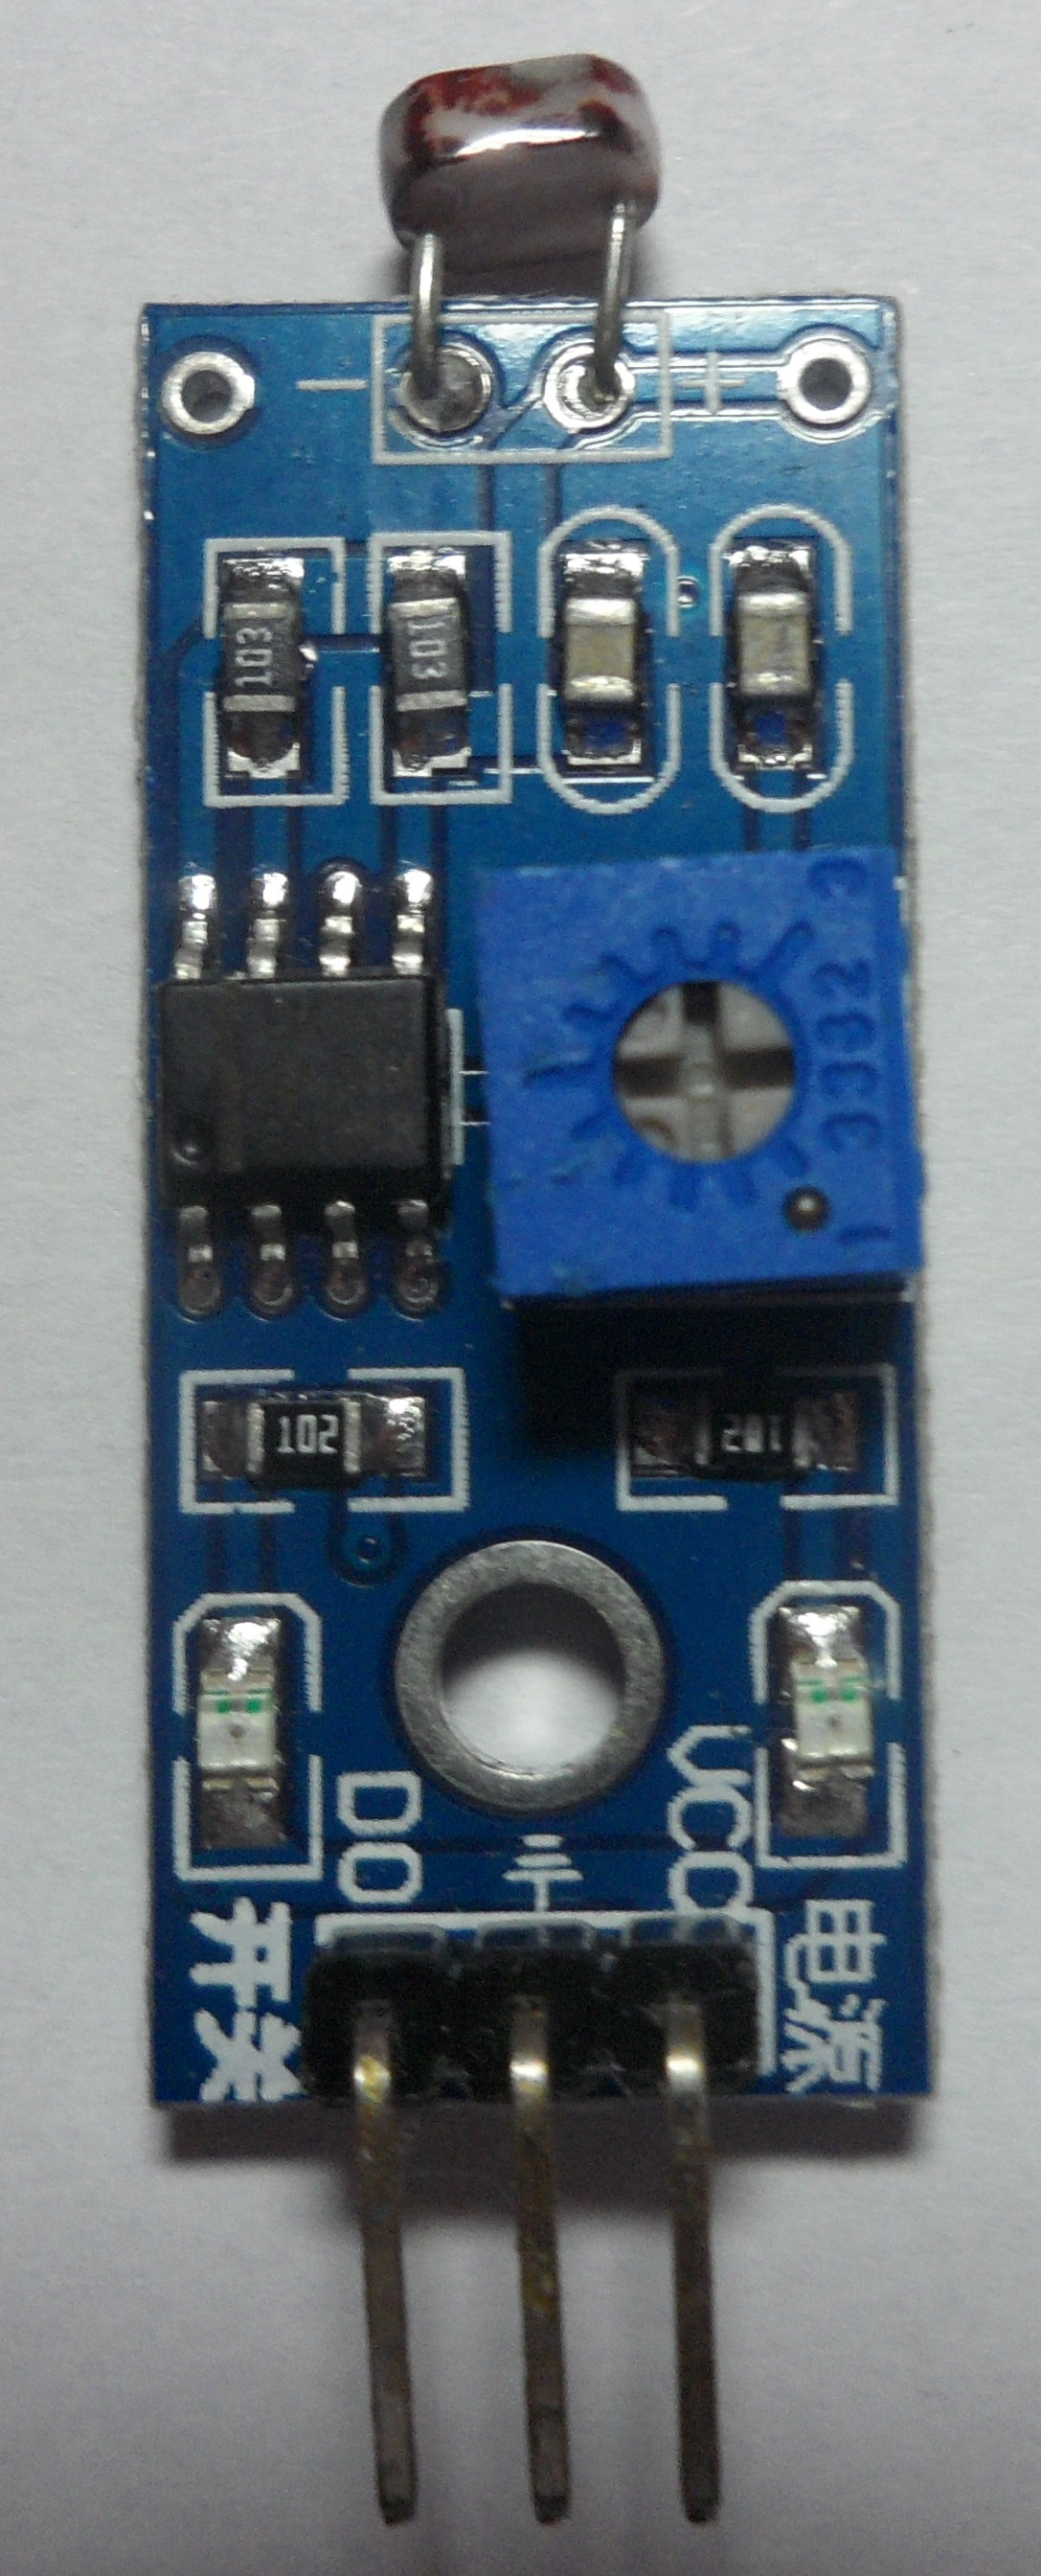
\includegraphics[width=0.2\textwidth]{figuras/luz}}
		\subfloat[Sensor de Ruido]{
			\label{f:ruido}
			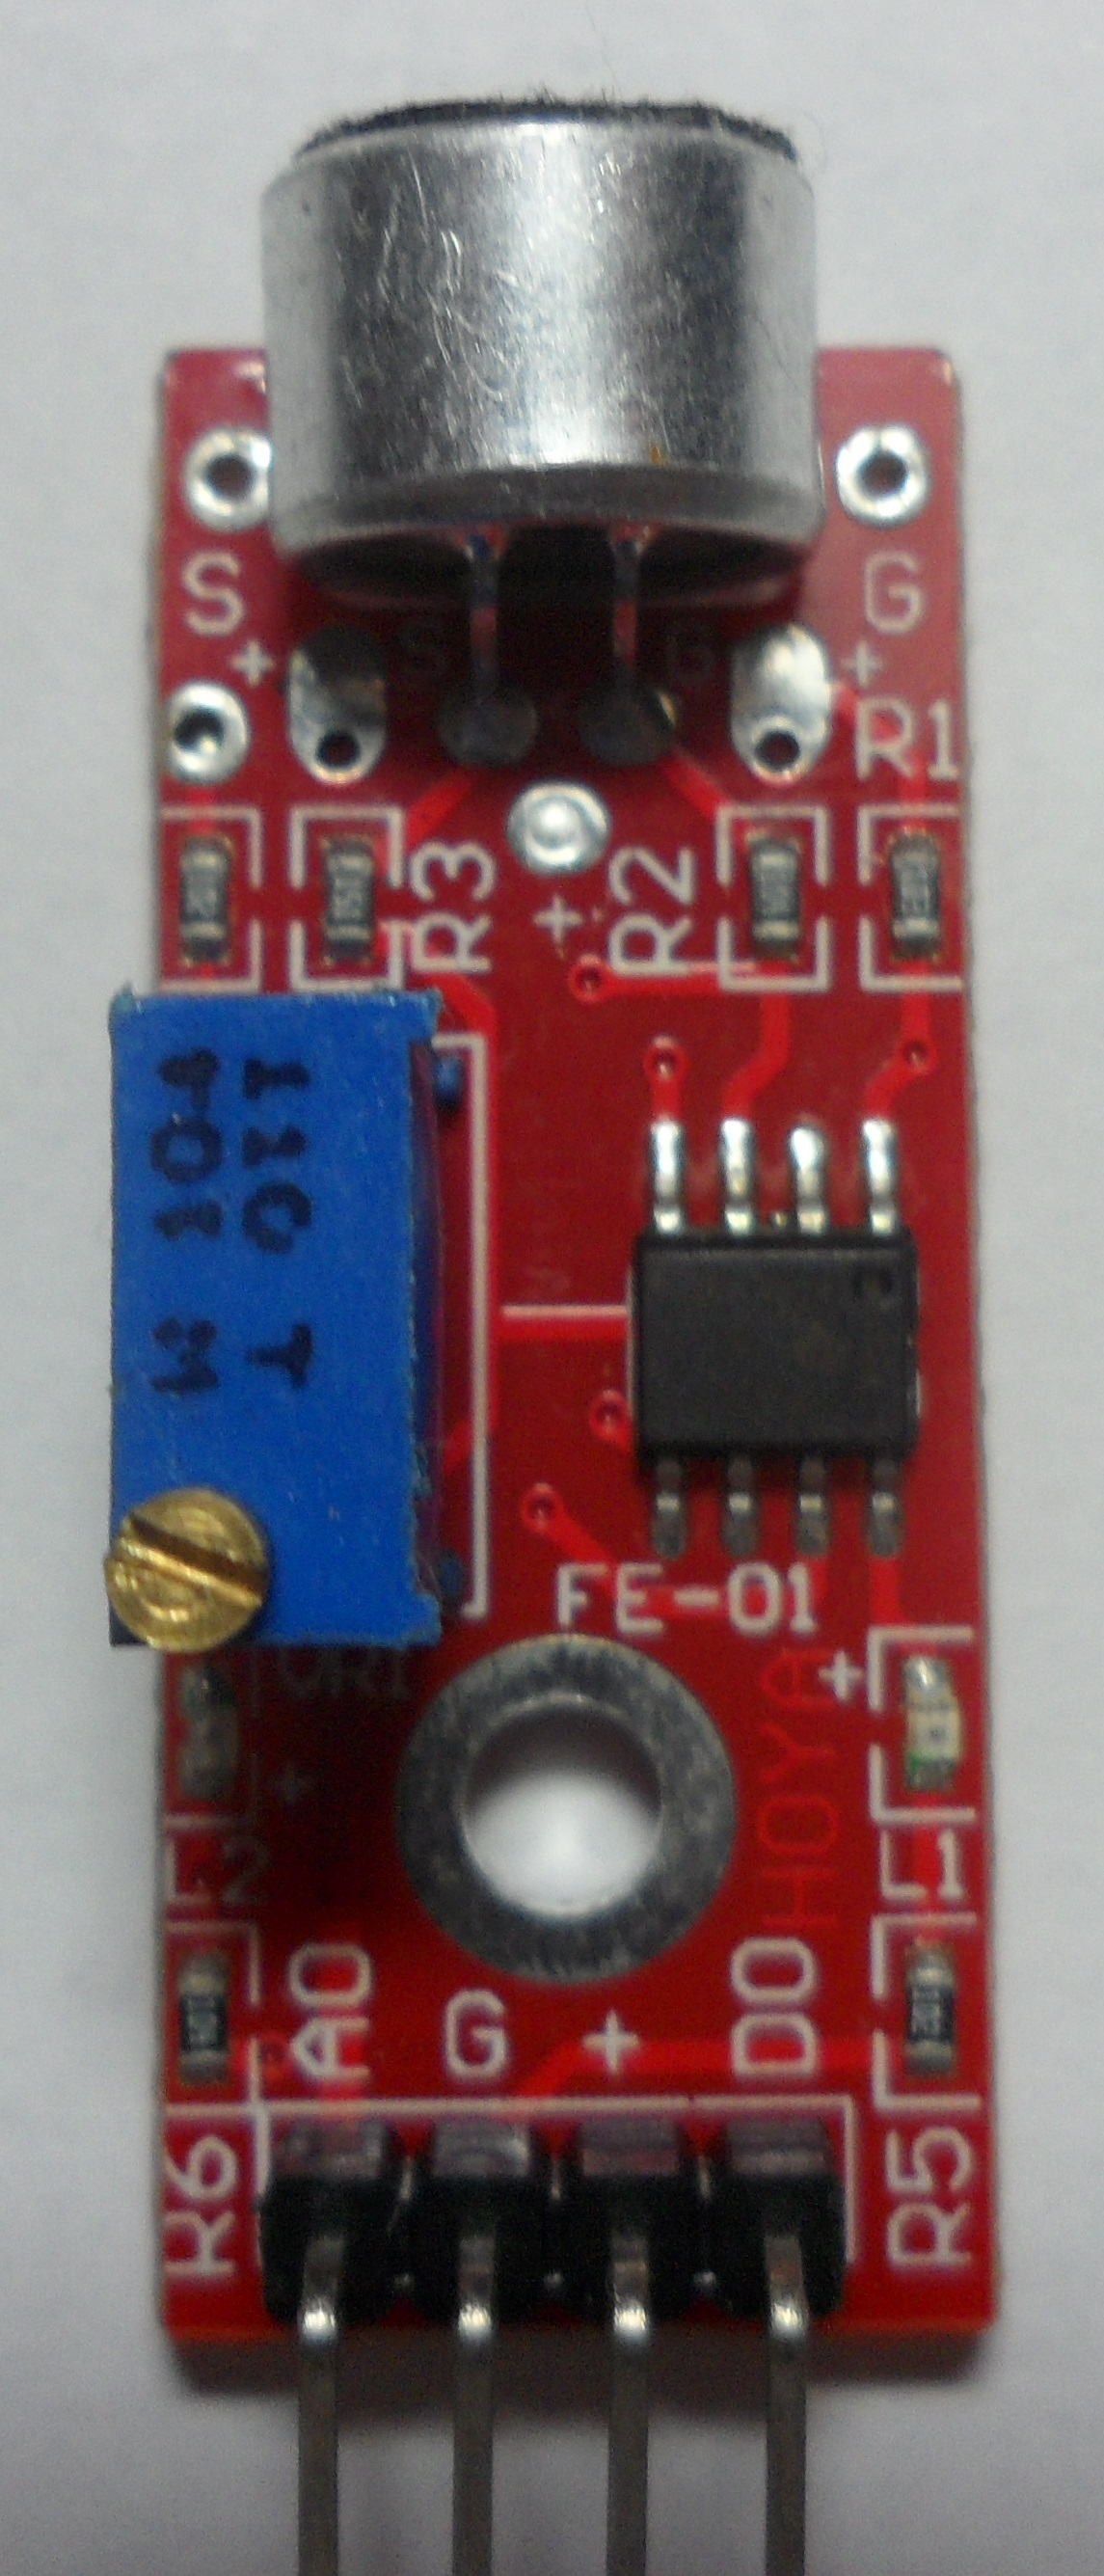
\includegraphics[width=0.2\textwidth]{figuras/noise}}
		\caption{Sensor de Luminosidad y Ruido}
		\label{f:sensores}
	\end{figure}
	
\end{itemize}

\textbf{Servidor:} El servidor que se va a utilizar para realizar las función de conexión entre el nodo y la la base de datos y entre el cliente y la conexión con el cliente a través de la aplicación web.

Las características de este servidor serán:

\begin{itemize}
	\item \textbf{CPU:} Intel i5 2500K a 3.3 GHz de funcionamiento.
	\item \textbf{Memoria:} 8 GB 1600 MHz DDR3.
	\item \textbf{Almacenamiento:} 2 TB de Almacenamiento, el que permitirá tener una base de datos bastante amplia.
	\item \textbf{S.O:} OSX El Capitan 10.11.6.
\end{itemize}

\textbf{Aplicaciones: } Aplicaciones que me han permitido realizar el montaje de todo el sistema.

Entre ellas están:

\begin{itemize}
	\item \textbf{Mamp:} Es una aplicación para montar un servidor web Apache y Mysql bajo los puertos 8888 para el web y 8889 para el Mysql.
	\item \textbf{MySQL Workbench} aunque es cierto que Laravel 5 gestiona la base de datos través de PHP se ha utilizado esta aplicación para poder gestionar la información almacenada en la base de datos.
	\item \textbf{PhpStorm } Un IDE de desarrollo para programar con PHP así como gestionar proyectos con Git.
\end{itemize}

\textbf{Cableado:} Distintos tipos de cableado para conectarlo todo.

\section{Montaje del Nodo Arduino DUE}

\setlength{\parindent}{5ex}El nodo para esta aplicación sera la microcontroladora con los módulos de sensores que enviaran información al servidor, para ello se realizara el montaje siguiendo el siguiente esquema:\\
\setlength{\parindent}{0ex}
\begin{figure}[!h]
	\centering
	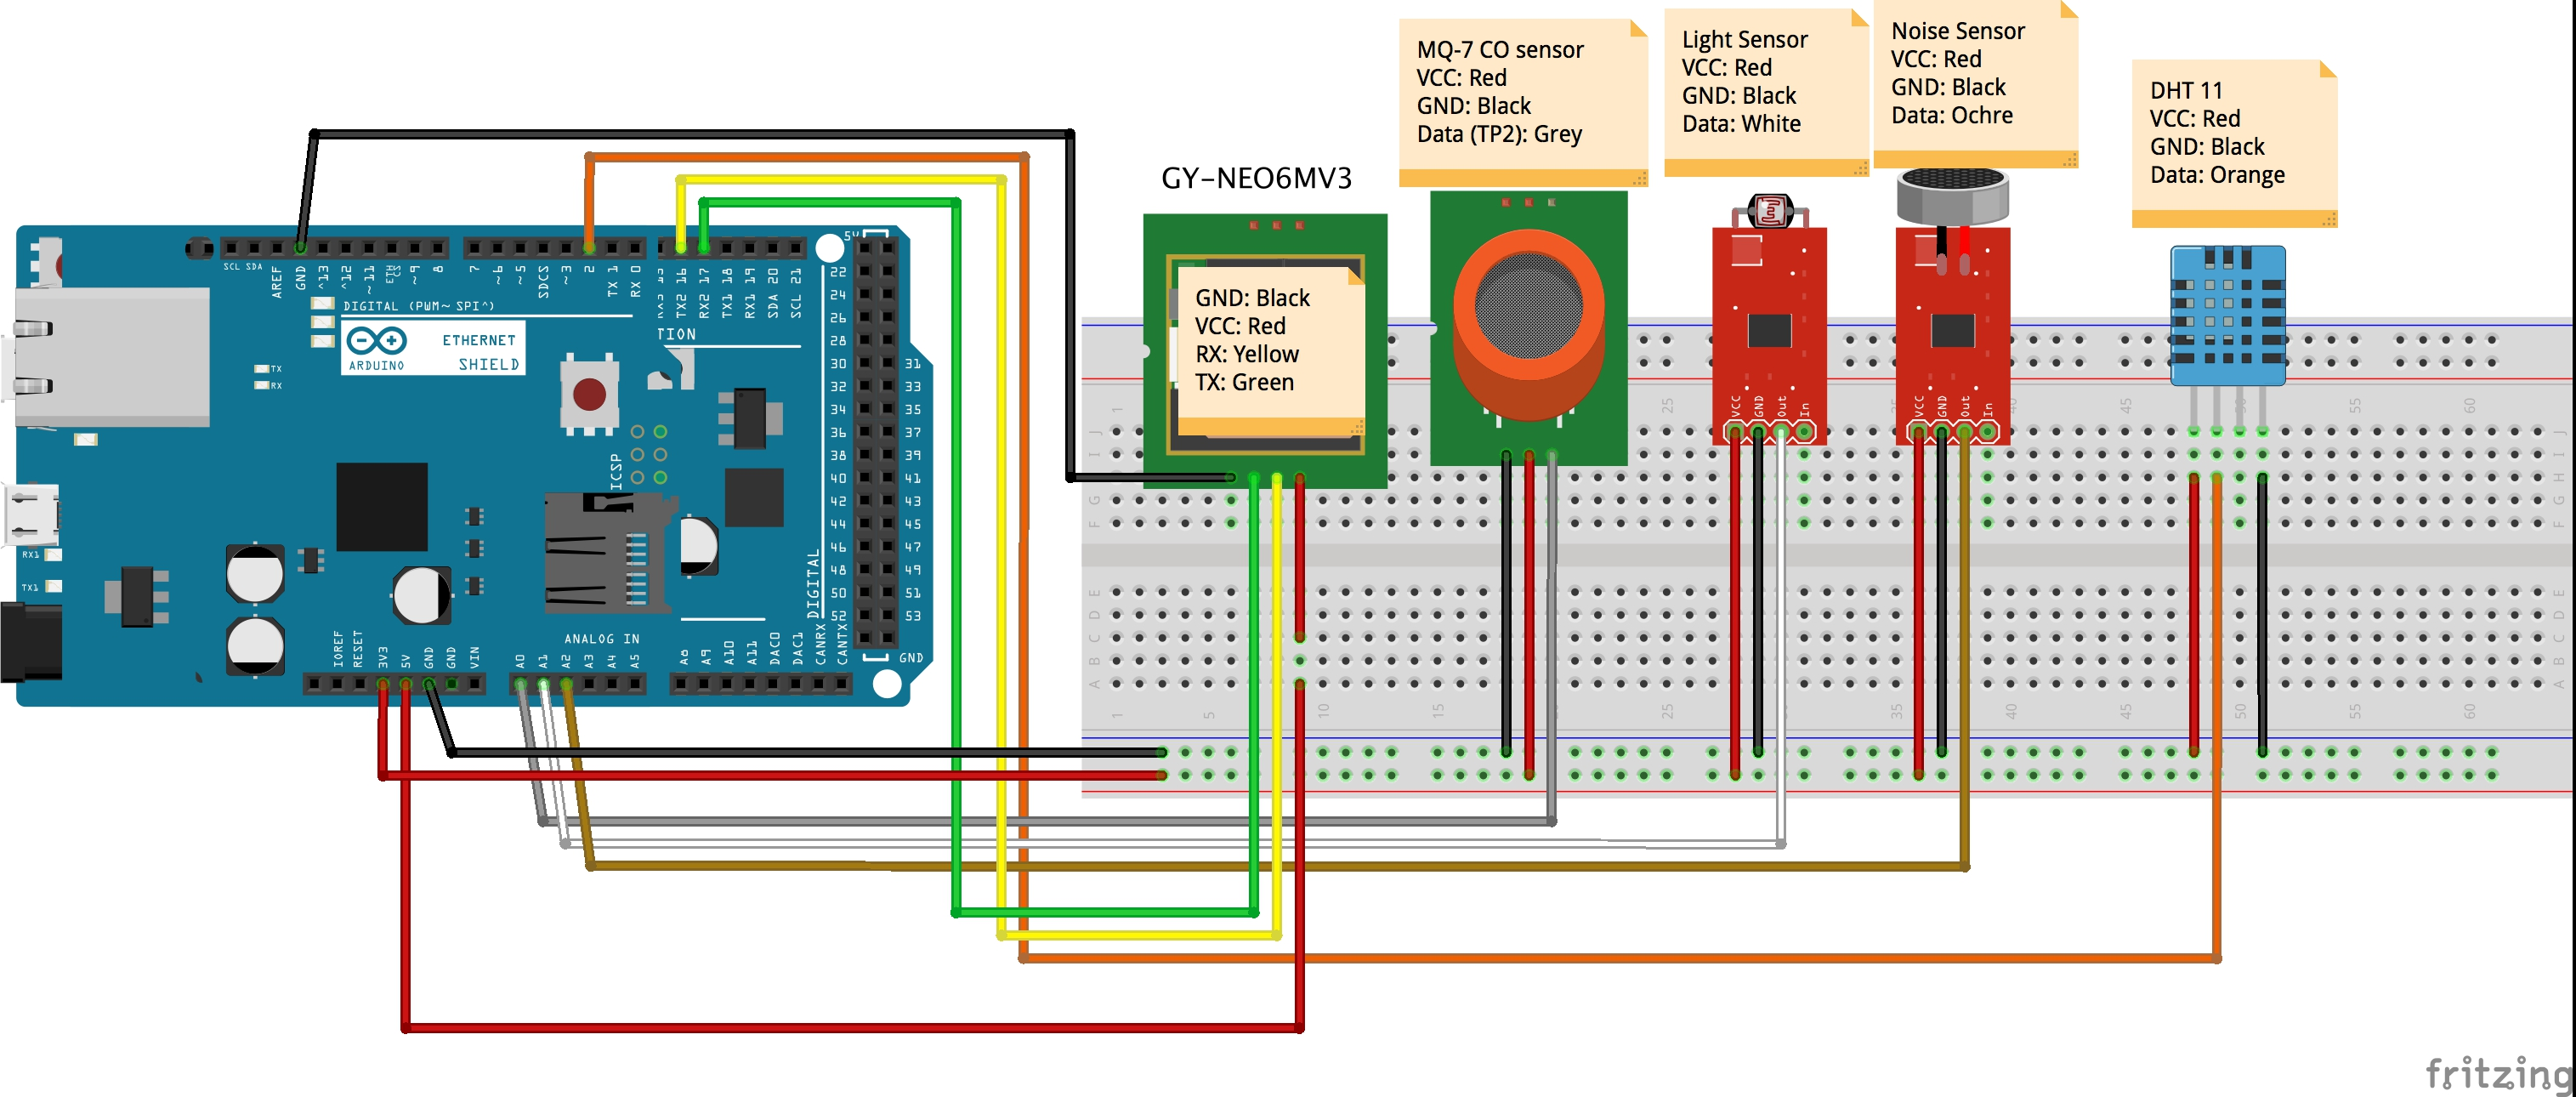
\includegraphics[width=0.9\linewidth]{figuras/ardschema}
	\caption{Esquema del montaje}
	\label{fig:imgdue}
\end{figure}

En la \textbf{Figura \ref{fig:imgdue}} se puede apreciar el esquema de las conexiones que he seguido para el montaje del nodo para que el código de la aplicación para Arduino recoja los valores correctamente.


Como se puede apreciar en el esquema el montaje es sencillo ya que no necesita electrónica adicional como resistencias u otros componentes electrónicos. Para conectar esto cada uno de los sensores, siguiendo el esquema, se conectara VCC (\textcolor{red}{Rojo}) a 3.3V ya que es el funcionamiento de cada uno de los sensores exceptuando el GPS que ira conectado a 5V ya que ha demostrado un mejor funcionamiento a ese voltaje y GND (\textcolor{black}{Negro}) para el negativo de los módulos, todos los sensores exceptuando el sensor de temperatura y humedad DHT11 que va a la entrada digital y el GPS que va conectado al Serial 2, van conectados a entradas analógicas (de A0 a A2).

Tener en cuenta que si se realiza en un Arduino UNO al ser una versión mas antigua las lecturas digitales se leen en un rango de 5V por lo que hay que diseñar un circuito especial para poder leer el GPS y el sensor DHT11 ya que estos devuelven una señal digital de 3.3V, para solucionar esto se tendrían que poner resistencias en el circuito con el fin de diseñar un sistema que aumente la señal a los 5V que necesita el Arduino UNO, que en este caso quedaría tal que así:

\begin{figure}[!h]
	\centering
	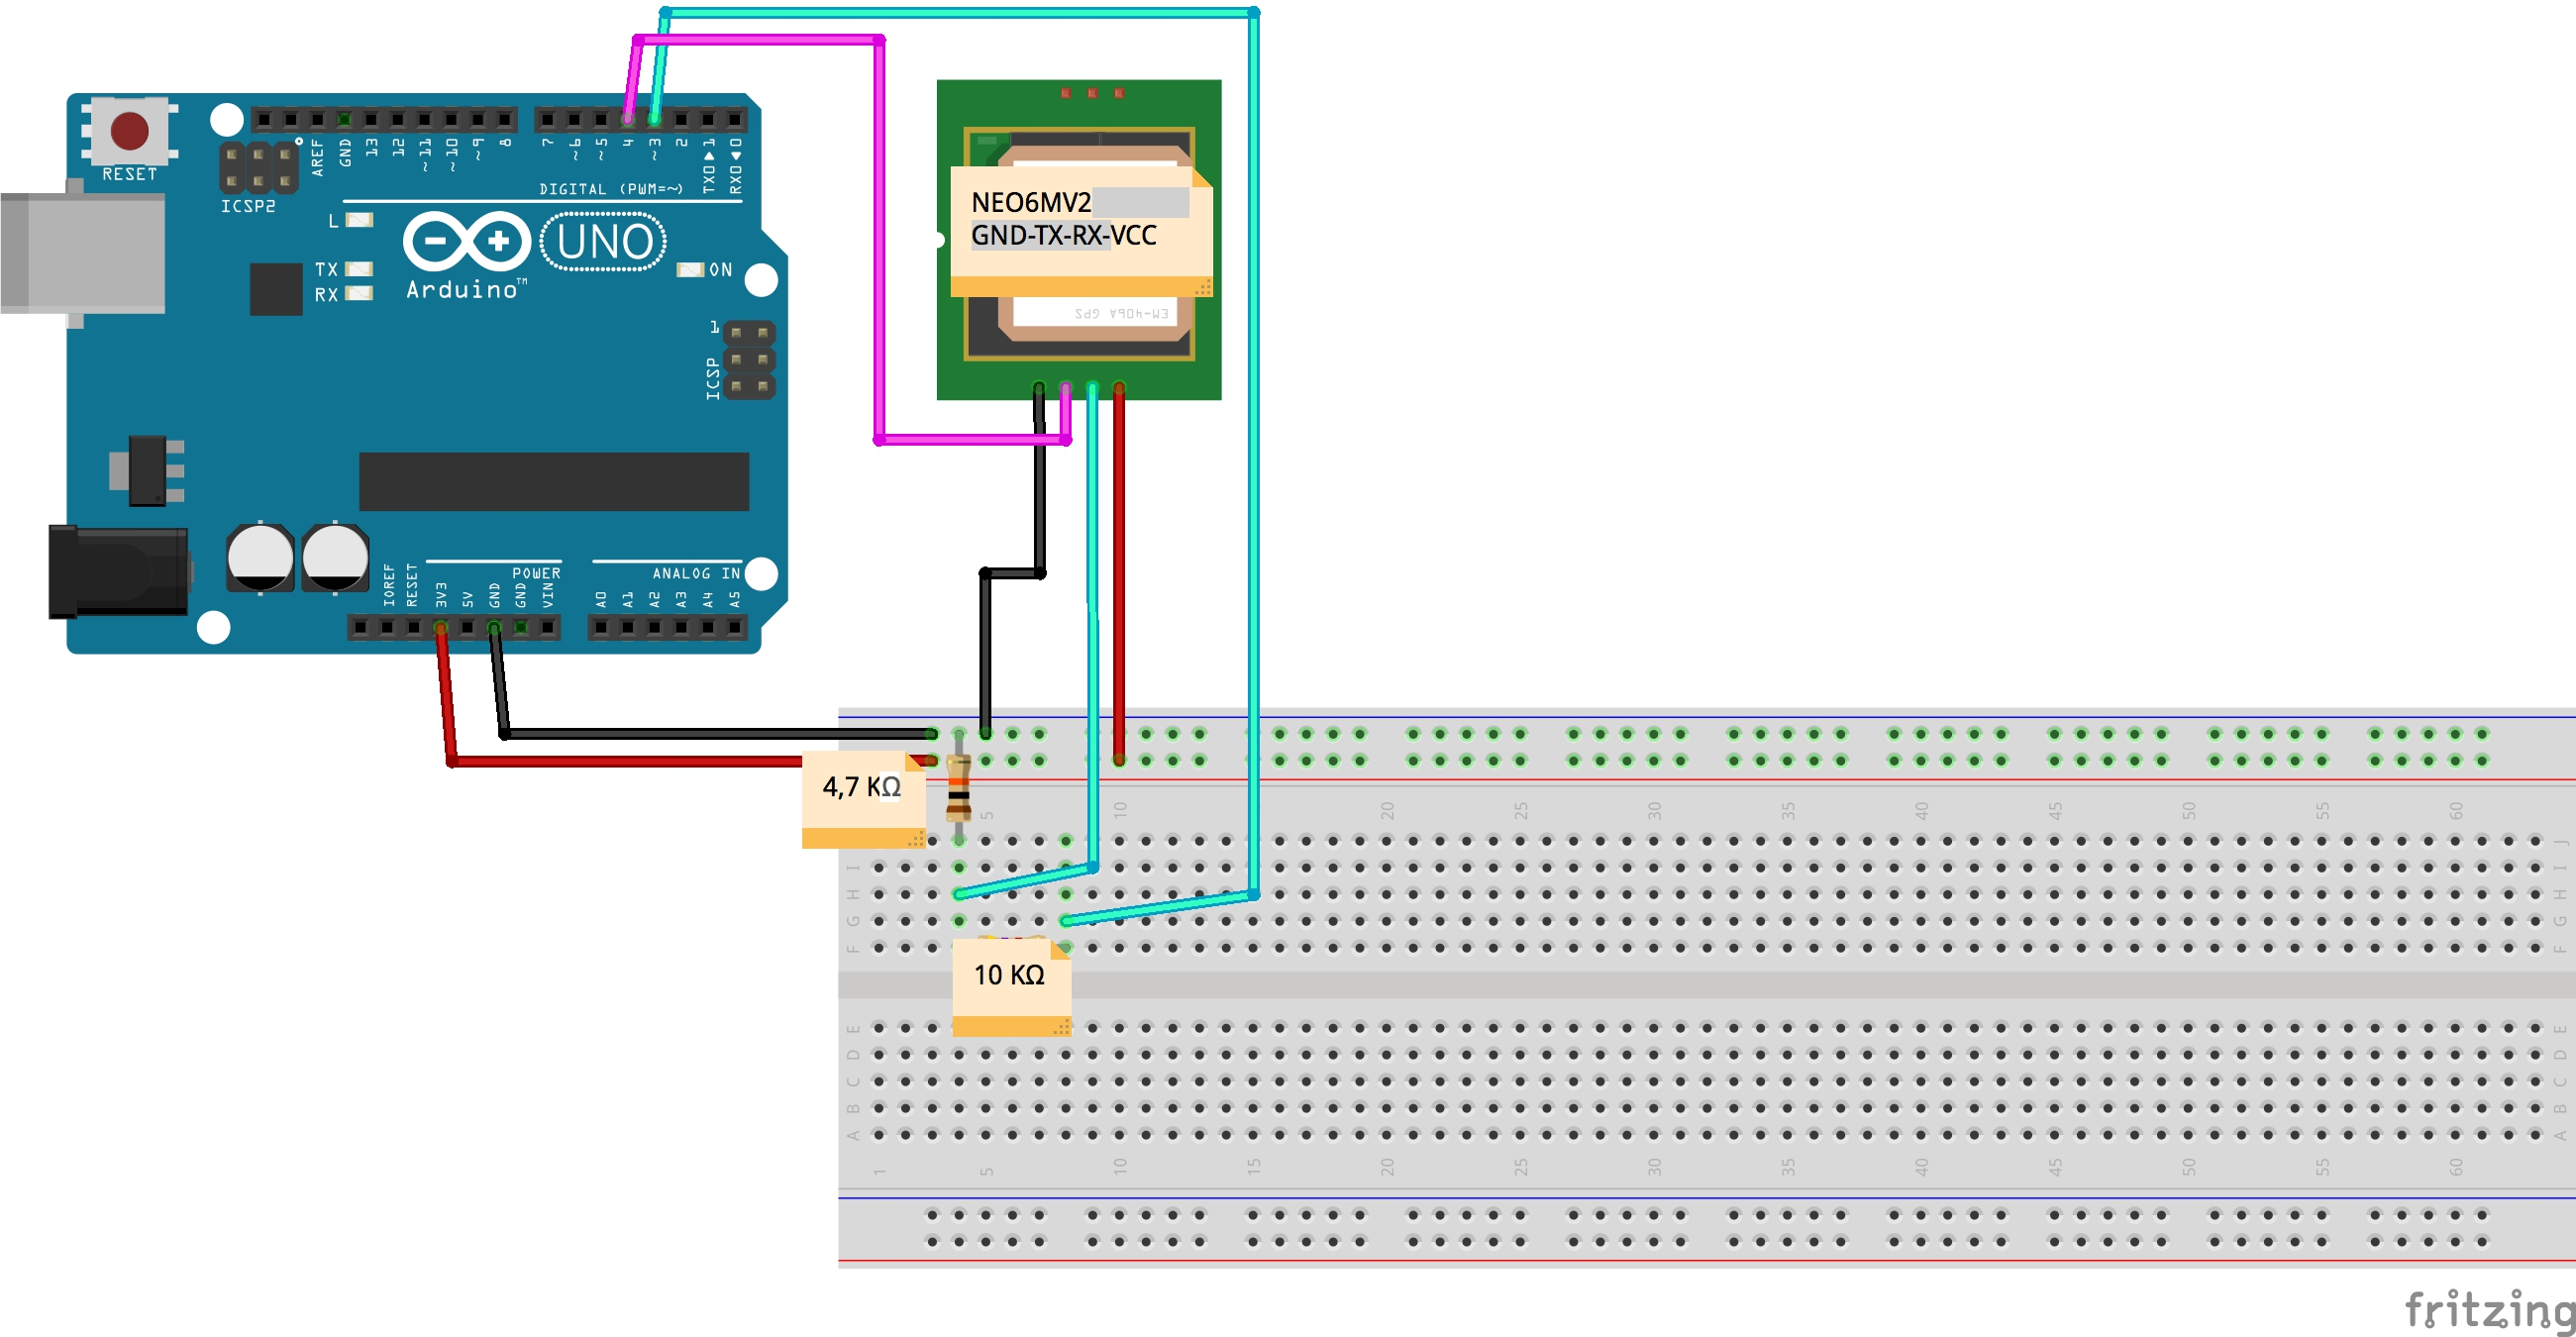
\includegraphics[width=0.9\linewidth]{figuras/unogps}
	\caption{Esquema del circuito para el GPS en el Arduino UNO}
	\label{fig:imgunogps}
\end{figure}

El circuito de la \textbf{Figura \ref{fig:imgunogps}} es un ejemplo de instalación para un modulo en Arduino UNO cuya respuesta en digital sea de 3.3V y sirve para otros módulos.

También comentar que los RX y TX de la trasmisión serie van conectados de manera invertida entre el GPS y el Arduino.

Este seria el montaje final de la electrónica de la controladora con todo el cableado y funcionando enviando la información al servidor.

\begin{figure}[!h]
	\centering
	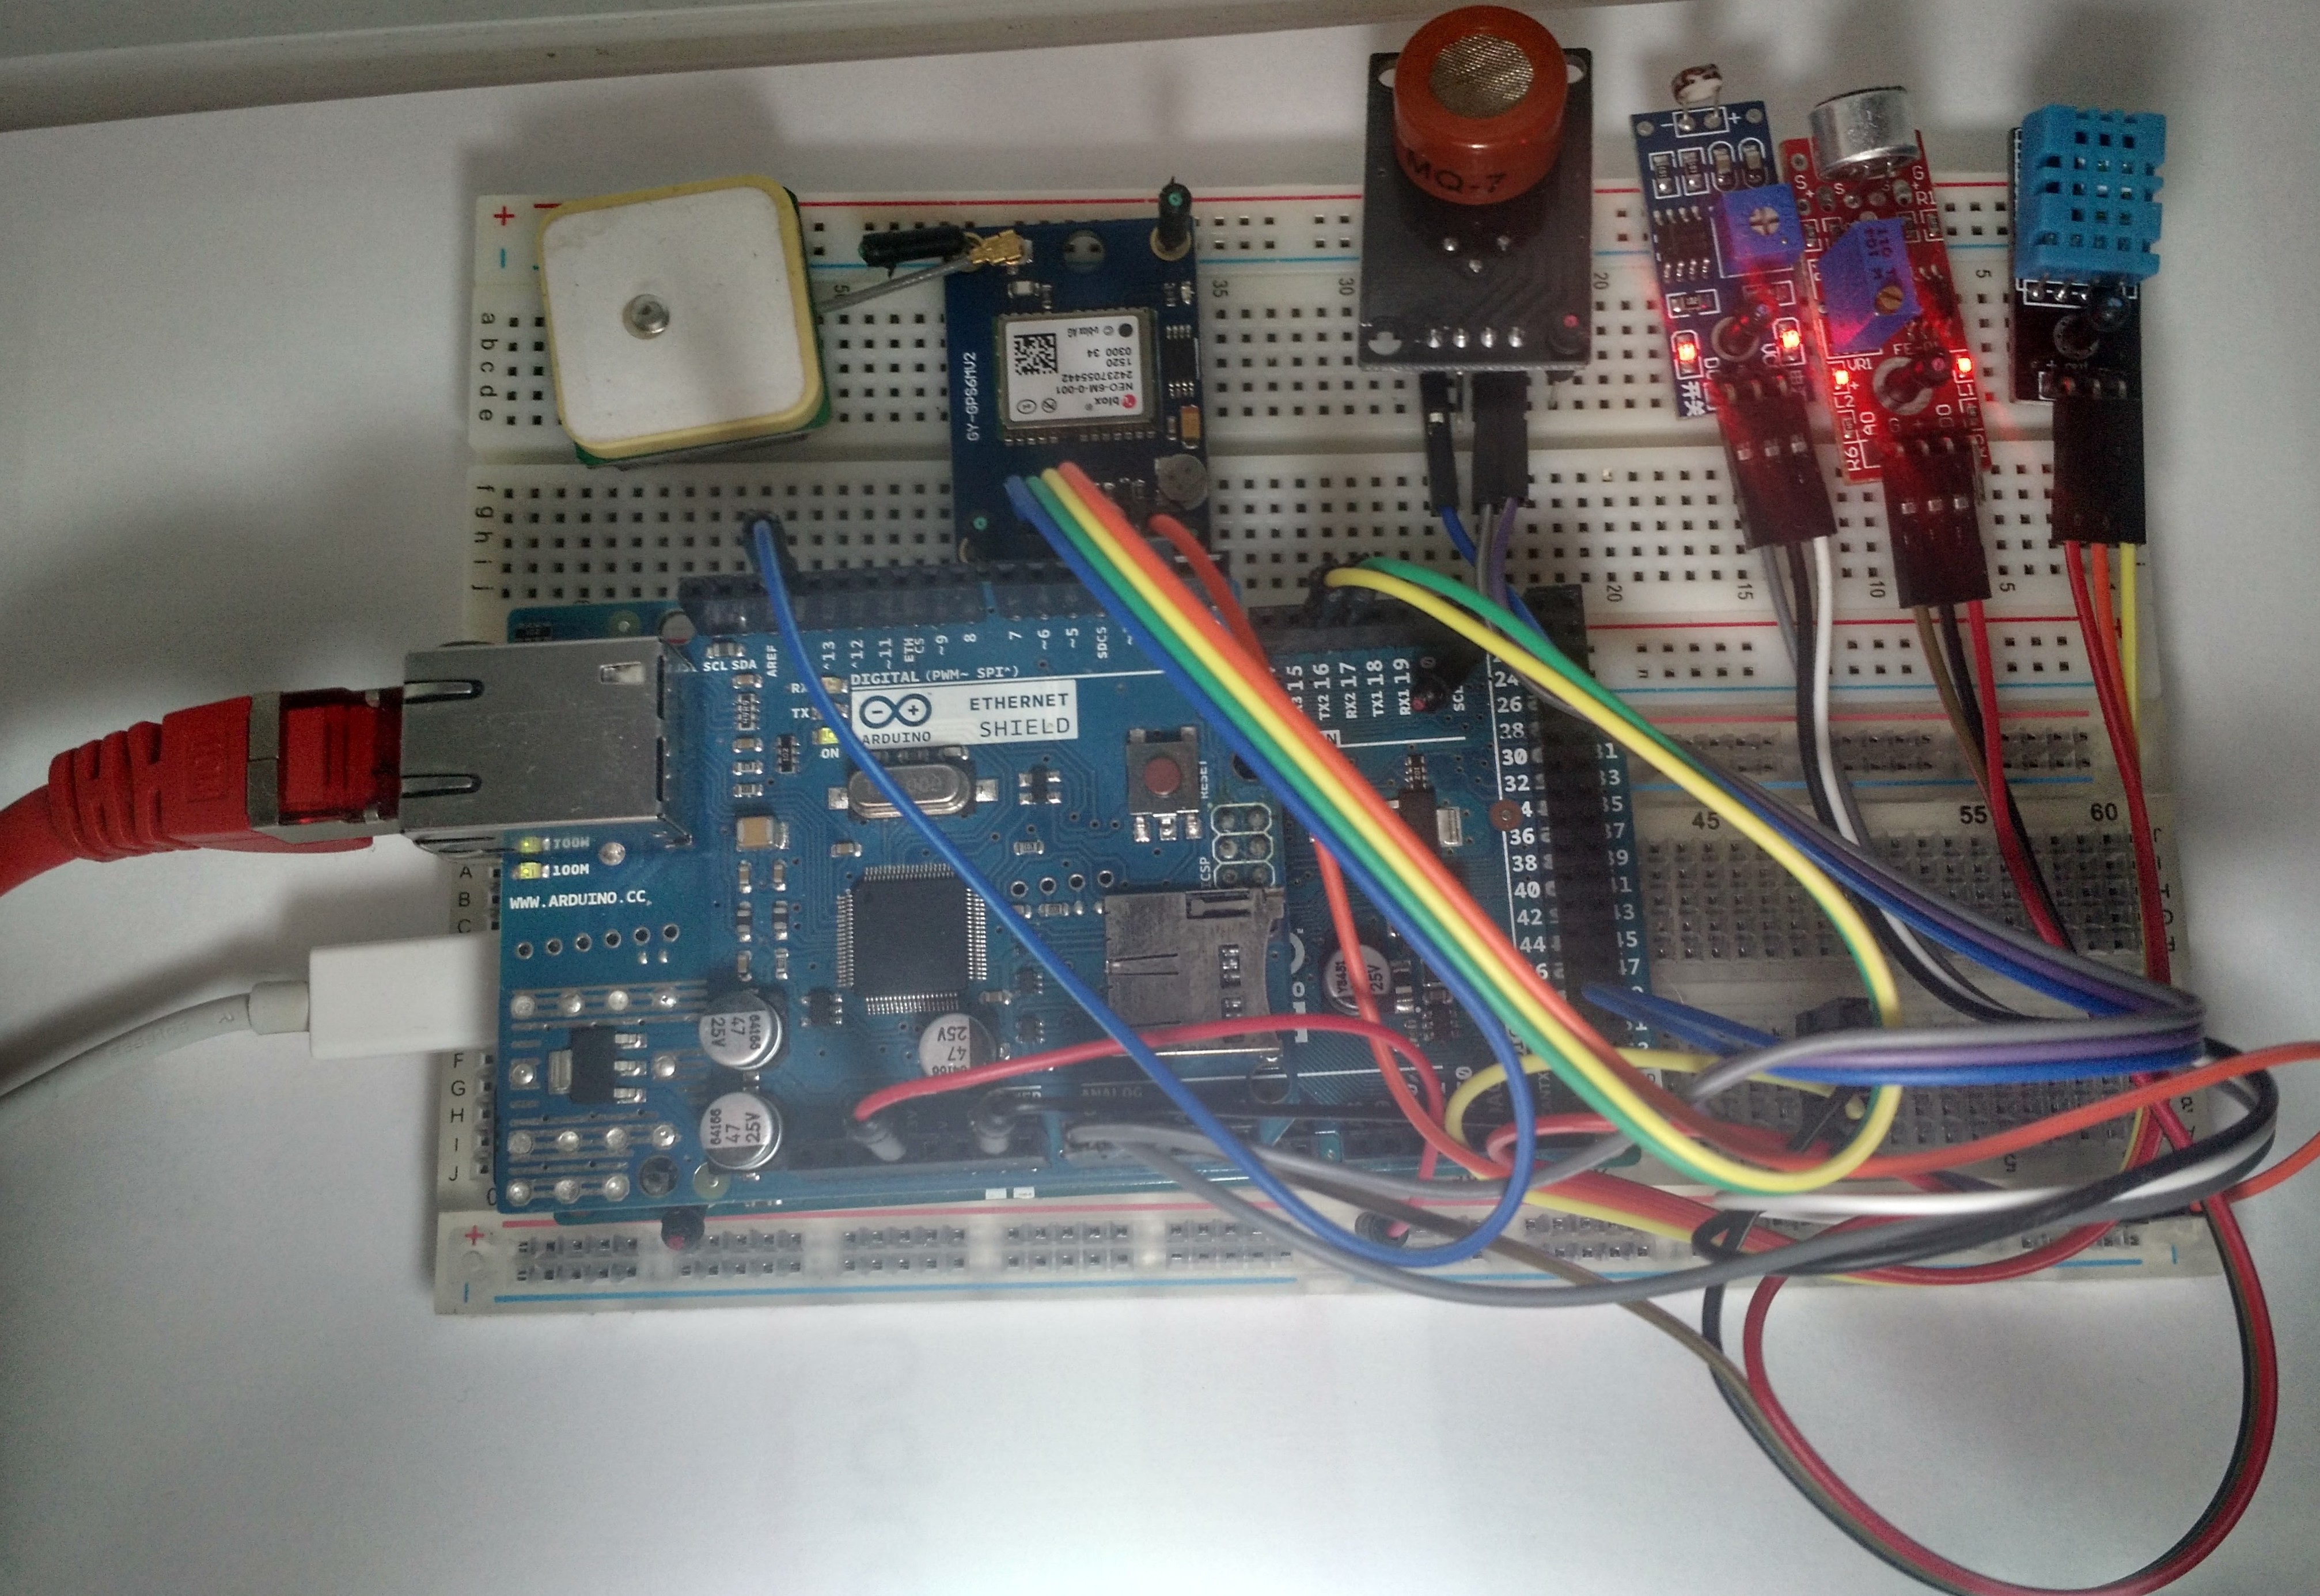
\includegraphics[width=0.7\linewidth]{figuras/montfin}
	\caption{Montaje final del nodo de sensores}
	\label{fig:montfin}
\end{figure}

Cada uno de estos sensores tendrá su función en el código de manera modular, así que es mas sencillo entender el funcionamiento del mismo.

\section{Programación de la Microcontroladora Arduino DUE}

\setlength{\parindent}{5ex}En este apartado se va a explicar cada una de las partes del código que utilizara el Arduino DUE, dicha parte realizara una función en la controladora por lo que el conjunto de todo el código realizara la función propuesta para este proyecto.
\setlength{\parindent}{0ex}

El código se puede descargar de la siguiente URL: \url{https://www.dropbox.com/s/qzzff1y6fqgluh8/project_1.3.1.ino?dl=0}\\

Esta es la parte de la configuración:

\begin{lstlisting}
/*
*  FILE:     project-v1.3.1.ino
*  AUTHOR:   David Rodriguez Martinez  davidrm146@gmail.com
*  VERSION:  1.3.1
*/
//Necessary Libraries
#include <Ethernet.h>
#include <SPI.h>
#include <TinyGPS.h>
#include "DHT.h"

//Config of the device
byte mac[] = { 0xDE, 0xAD, 0xBE, 0xEF, 0xFE, 0xED };
TinyGPS gps;
#define DHTPIN 2  
#define DHTTYPE DHT11  
DHT dht(DHTPIN, DHTTYPE);
IPAddress ip(192, 168, 1, 102);
EthernetClient client;
String data;
void setup()
{  
	Serial.println("EXECUTING setup");
	Serial.begin(9600);
	Serial2.begin(9600);
	if (Ethernet.begin(mac) == 0) {
		Serial.println("Failed to configure Ethernet using DHCP");
		Ethernet.begin(mac, ip);
	}
	delay(1000);   // A Small delay for avoid errors
}
\end{lstlisting}

Antes de entrar al código se implementaran las librerías para el funcionamiento de los módulos, en este caso lo que hacen es traducir la información para que pueda ser manipulada de manera mas fácil. las librerías son:

\begin{itemize}
	\item \#include <Ethernet.h>: Permite gestionar la conexión a la red.
	\item \#include <SPI.h>: Permite al Arduino DUE comunicarse con la Shield de Ethernet.
	\item \#include <TinyGPS.h> Esta librería traduce el NMEA data en valores legibles sin necesidad de manipular la cadena de hexadecimales recibida.
	\item \#include 'DHT.h':  Esta librería traduce la información recibida por el sensor DHT11, solo hace falta configurar que pin es el que recibirá la información y que tipo de sensor se va a utilizar ya que la librería configura automáticamente la comunicación con el sensor.
\end{itemize}

Esta es la configuración de Arduino encapsulada en la definición de SETUP en esta parte del código se definirá la comunicación vía serie para el modulo GPS conectado al serial 2 a 9600 baudios aunque aplicando una serie de cadenas hexadecimales en el arranque del programa escritas en el GPS vía serie.
También se configurara la conexión serie que le pertenece al puerto USB para poder observar la información que envía cada vez que se repita el bucle del programa con el fin de poder debugguearlo en caso de algún problema o fallo de los componentes.\\

\begin{lstlisting}
	if (Ethernet.begin(mac) == 0) {
		Serial.println("Failed to configure Ethernet using DHCP");
		Ethernet.begin(mac, ip);
	}
\end{lstlisting}
Esta parte es la conexión a la red, en este caso por DHCP que solo hace falta asignarle la MAC al dispositivo o si falla asignar manualmente una dirección IP que corresponderá a la de la red interna.

Una vez configurado todo el programa ya estará listo para leer la información que recojan los módulos de sensores asi que se dieñara el siguiente codigo para realizar dicha lectura en la definición del LOOP el cual se ejecutara indefinidamente:\\

\begin{lstlisting}
void loop(){
	Serial.println("EXECUTING LOOP");
//***************GPS CODE*********************
	bool newData = false;
	unsigned long chars;
	unsigned short sentences, failed;
		for (unsigned long start = millis(); millis() - start < 1000;){
			while (Serial2.available()){
				char c = Serial2.read();
				if (gps.encode(c))newData = true;
			}
		}
	float flat, flon;
	unsigned long age;
	gps.f_get_position(&flat, &flon, &age);
	Serial.print("LAT=");
	Serial.print(flat == TinyGPS::GPS_INVALID_F_ANGLE ? 0.0 : flat, 6);
	Serial.print(" LON=");
	Serial.print(flon == TinyGPS::GPS_INVALID_F_ANGLE ? 0.0 : flon, 6);
	Serial.print(" SAT=");
	Serial.print(gps.satellites() == TinyGPS::GPS_INVALID_SATELLITES ? 0 : gps.satellites());
	Serial.print(" PREC=");
	Serial.println(gps.hdop() == TinyGPS::GPS_INVALID_HDOP ? 0 : gps.hdop());

//The next variable keeps the information collected by the sensors
	data = 
		"board_id=" +  getID()  +
		"&temp=" +  getTemperature()  + 
		"&hum=" + getHumidity() +
		"&gas="+ getGas() + 
		"&noise=" + getNoise() +
		"&luz="+ getLight() + 
		"&poslat=" + String(flat, 6) + 
		"&poslon=" + String(flon, 6);

//Debug function, this string works
//data ="board_id=1&temp=23&hum=43&gas=53&noise=54&luz=55&poslat=63&poslon=73";
		displayData(data);
//This function is for send information to the server
		sendDataGet(data);
delay(60000);
}
\end{lstlisting}

En esta parte del código se realizan 3 funciones, la lectura del GPS, el envío de la cadena que contiene las funciones que recogen de datos de los sensores y el delay que establecer un periodo de envío de información con el fin de evitar saturar la red.\\

\begin{lstlisting}
	for (unsigned long start = millis(); millis() - start < 1000;){
		while (Serial2.available()){
			char c = Serial2.read();
			if (gps.encode(c))newData = true;
		}
	}
\end{lstlisting}

Esto recogerá la información del gps en formato de NMEA data pero gracias a la librería TinyGPS.h que nos traduce directamente sin tener que editar manualmente el NMEA data, la información obtenida del GPS leyendo el Serial2 del Arduino DUE devolviendo nos información del GPS, en este caso nos interesa \textbf{flat} y \textbf{flon} que son las coordenadas que recoge el GPS.

 Los Serial.print están para mostrar la información obtenida ya que este no conecta al instante al satélite como ya se vera en el funcionamiento del vídeo mas adelante.

También se recoge la información para enviar al servidor en la variable \textbf{data} en la que se llaman las funciones que recogerán la información, es importante que el formato de la cadena sea como esta especificado en los comentarios, siguiendo el nombre de las variables ya que si no están bien nombrados la función del servidor que se encarga de recoger la información no funcionara y no se podrá realizar la inserción a la base de datos. Este es un ejemplo de como debería ser definida:\\

\begin{lstlisting}
		data="board_id={id} +
			&temp={temperatura} +
			&hum={humedad} +
			&gas={medicion del gas} +
			&noise={ruido ambiental} +
			&luz={luminosidad} +
			&poslat={latitud} +
			&poslon={longitud}";
\end{lstlisting}

Y por ultimo una delay o pausa que evitara que el Arduino esté enviando información constantemente de 1 minuto (60000 milisegundos)

Una vez explicado el bucle se explicaran las funciones que se ejecutan en la variable de datos ya que son las que recogen la información ambiental de la zona donde esta situado:\\

\begin{lstlisting}
String getTemperature() {
	float t = dht.readTemperature();
	float f = dht.readTemperature(true);
	if (isnan(t) || isnan(f)) {
		Serial.println("Failed to read Temperature from DHT. . .");
		return "0";
	}
	return String(t, 2);
}

String getHumidity() {
	float h = dht.readHumidity();
	if (isnan(h)) {
		Serial.println("Failed to read Humidity from DHT. . .");
		return "0";
	}
	return String(h, 2);
}

String getGas() {return String(analogRead(A0));}

String getLight() {return String(analogRead(A1));}

String getNoise() {return String(analogRead(A2));}

String getID() {return "1";}
\end{lstlisting}

En las funciones \textit{getTemperature} y \textit{getHumidity} se puede apreciar que gracias a la librería dht.h se realiza la conexión y lectura de la información del sensor sin tener que crear código adicional para controlar este sensor. Sobre las demás funciones son lecturas analógicas de las mismas que nos dan unos valores normales en su rango de 1 a 1024. Y la ultima sirve para establecer la id en la que esta registrada en la base de datos, este numero debe coincidir con su controladora como ya se explicará mas adelante.

Una vez ya esta explicado el código se explicara la llamada a la web la cual realizara la inserción a la bd, este es su código:

\begin{lstlisting}
void sendDataGet(String data) {
	if (client.connect("192.168.1.16",8888)){
		client.print("GET /call?");
		client.println(data);
		client.println("HTTP/1.1");
		client.println("Host: 192.168.1.16");        
		client.println("Connection: close");
		client.println();
	}
	if (client.connected()) { 
		client.stop();
	}
}
\end{lstlisting}

Esta función realiza la petición GET al servidor web el cual se configurara con la ip y el puerto en el que esté trabajando el servidor, puede ser publica o privada por lo que el Arduino puede trabajar en Internet aunque es mucho mas inseguro para la aplicación pues uno de sus puntos débiles es que el Arduino no tiene capacidad para la encriptación y tampoco tiene soporte para peticiones HTTPS por lo que una gran falla de este proyecto son los ataques \textit{man in the middle}, la llamada corresponde a una petición a la web "call?información..." en la cual se obtendrá la información en forma de JSON y sera almacenada den la BD.

La llamada o dirección del servidor web quedaría algo tal que así: 

\begin{lstlisting}
	192.168.1.16:8888/call?board_id={id}&temp={temperatura}&hum={humedad}&gas={medicion del gas}&noise={ruido ambiental}&luz={luminosidad}&poslat={latitud}&poslon={longitud}
\end{lstlisting}

Este es el código de la pagina web PHP que recogerá los datos en formato JSON y los guardara en la base de datos, todo ello realizado en Laravel 5.

\begin{lstlisting}
 public function setData(){
		 $getData = Request::all();
		 data::create($getData);
		 if (!$this->active){$this->setWorking(Request::get('board_id'));}
		 return $getData;
 }
\end{lstlisting}

La función \textit{\$getData = Request::all();} recoge toda la información que reciba en un GET o POST y lo introduce en la variable en formato JSON luego se ejecutaría el controlador de data la función \textit{data::create(\$getData);} de ahí la importancia que las variables introducidas en la variable data de Arduino estén nombradas como se ha especificado ya que en la BD se han de nombrar igual para que las entradas puedan ser introducidas correctamente.

Este es el resultado del JSON cuando se recibe la petición GET en la función:

\begin{figure}[!h]
	\centering
	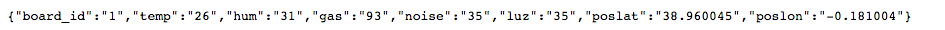
\includegraphics[width=1.0\linewidth]{figuras/jsonstring}
	\caption{String JSON generada por la petición GET de Arduino}
	\label{fig:montfin}
\end{figure}

Una vez configurado esto ya se podría dejar la microcontroladora trabajando para la recolección de datos.

\section{Instalación del Servicio WEB}

Para la instalación en este caso se requiere de un Servidor WEB con la funcionalidad de PHP5 y un SGBD (en este caso MySQL) añadido, en este proyecto se ha utilizado el servidor MAMP que es una aplicación de OSX que dispone de estas características el cual se va a utilizar para almacenar la información.

Para la instalación de la aplicación en el servidor se ha de descargar de este enlace el cual contiene un paquete de archivos que contienen la aplicación: 

\url{https://www.dropbox.com/sh/nf8qp6jtqgrqb9d/AACmTXwt8dyTvCTKeraueG9oa?dl=0}\\

Una vez descomprimido se le aplican los permisos lectura y escritura al usuario y lectura a otros (\texttt{sudo chmod 744 tfg-laravel}) desde la terminal y se configura el directorio del servidor WEB:
\clearpage

\begin{figure}[!h]
	\centering
	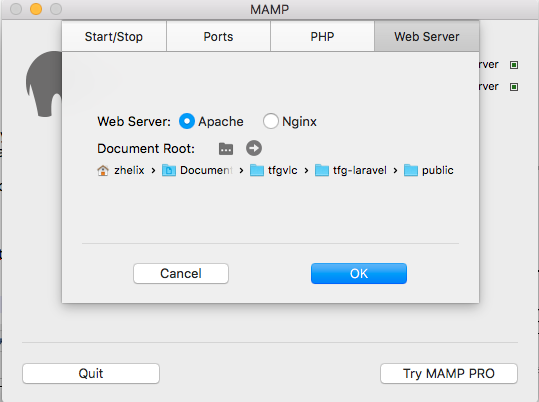
\includegraphics[width=0.7\linewidth]{figuras/confmamp}
	\caption{Configuración del Servidor MAMP}
	\label{fig:confmamp}
\end{figure}

El la ventana de la \textbf{Figura \ref{fig:confmamp}} se muestra la configuración básica del directorio de la aplicación, que en este caso ha sido alojado en la carpeta de usuario, los demás parámetros se dejaran por defecto como es el puerto HTTP que lo configurara al 8888 y el servidor de Base de Datos que sera el 8889.

